\section{AMIDST Model Class}

\subsection{Introduction}

One of the main goals of this project [] was the definition of a general model class which the following features: (i) it has to be applicable to the three main use-cases; (ii) it should be general enough to apply to other future similar use-cases;  (iii) and it should contain certain structure that can be exploited to make this model class valid for scalable inference and learning in massive data streams. 

With these three aims in mind,  we started the definition of the general model class by finding commonalities between the different models presented in Section \ref{Section:PreliminaryModels}.  To try to elicit these commonalities between the proposed models for the three use-cases, we  introduce some new ``graphical'' notation to ease this process. This new graphical notation is based on the use of subnetworks modules (?), they are represented by square boxes and represents a subset of nodes with some kind of interconnection between them (when looking at the examples, we think this concept will be much clear). Following the same notation we used for nodes, square boxes rounded by dashed lines refers to a subnetwork which is not observable (i.e. composed by hidden variables); square boxes rounded by continuous lines refers to a subnetwork where the nodes are observed; when the square box is coloured, it means that all the nodes of the subnetwork are discrete (green color) or continuous (blue color). Square boxes can also be nested to represent smaller subcomponents inside a bigger subcomponent. In Figure ? we give a visual description of this notation. 

\begin{figure}
\begin{center}
\caption{\label{Figure:ModelClass0} Graphical Notation}
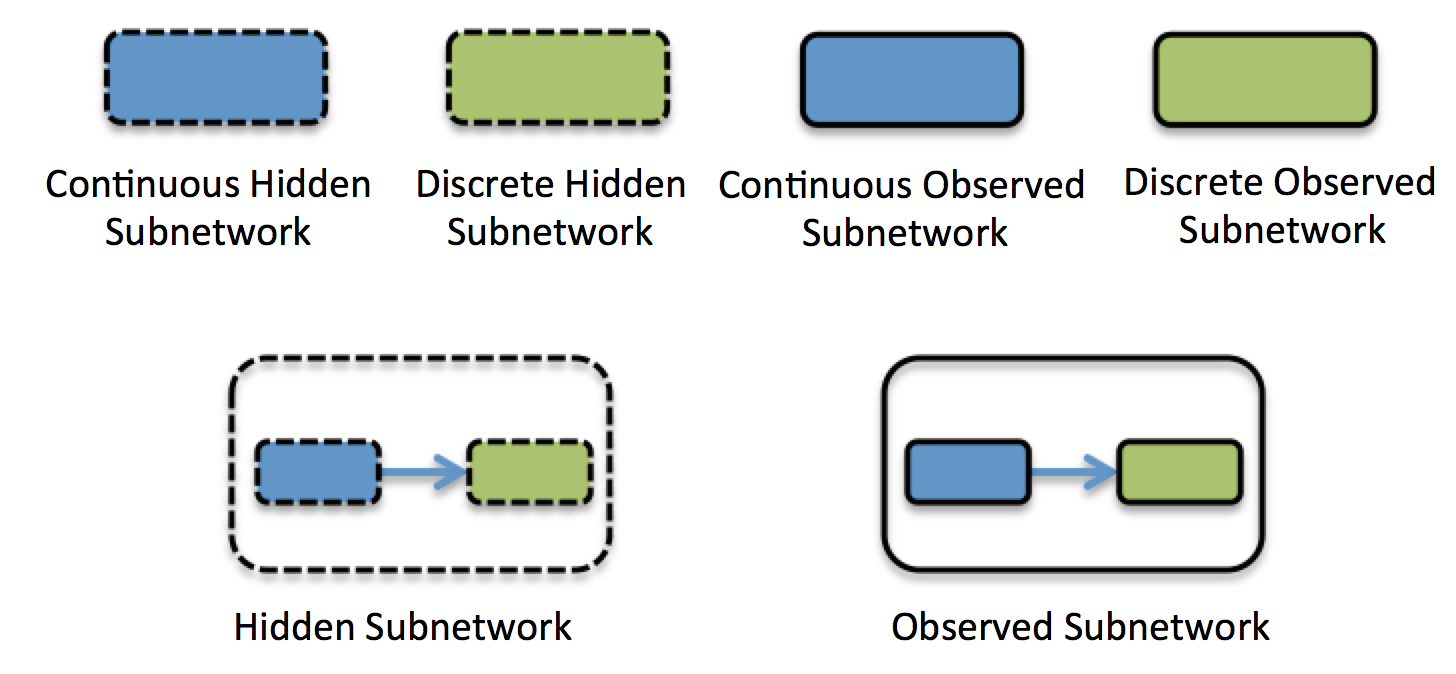
\includegraphics[scale=0.4]{./figures/ModelClass0}
\end{center}
\end{figure}

In this new step, we are going to present again the models of the three use-cases but using now this previously introduced notation. 

\subsubsection*{Daimler Model Class}

\begin{figure}
\begin{center}
\caption{\label{Figure:DaimlerModelClass} Daimler Model Class}
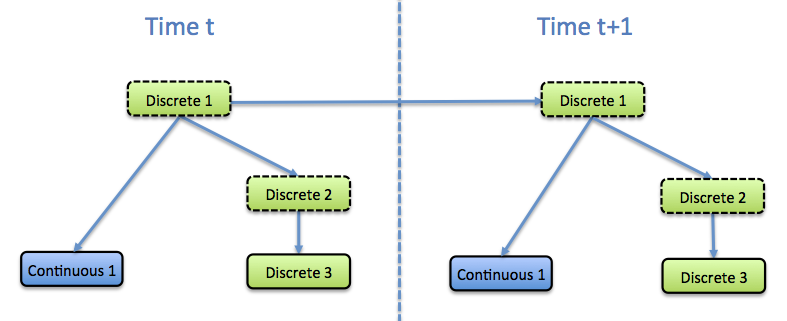
\includegraphics[scale=0.4]{./figures/DaimlerModelClass}
\end{center}
\end{figure}

\subsubsection*{Verdande Model Class}

\begin{figure}
\begin{center}
\caption{\label{Figure:VerdandeModelClass} Verdande Model Class}
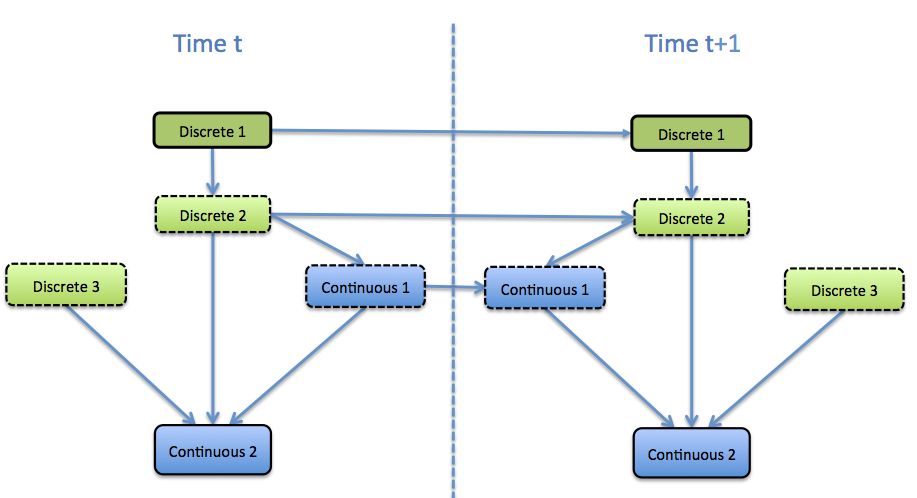
\includegraphics[scale=0.4]{./figures/VerdandeModelClass}
\end{center}
\end{figure}


\subsubsection*{Caja Mar Model Class}

\begin{figure}
\begin{center}
\caption{\label{Figure:CajaMarModelClass} CajaMar Model Class}
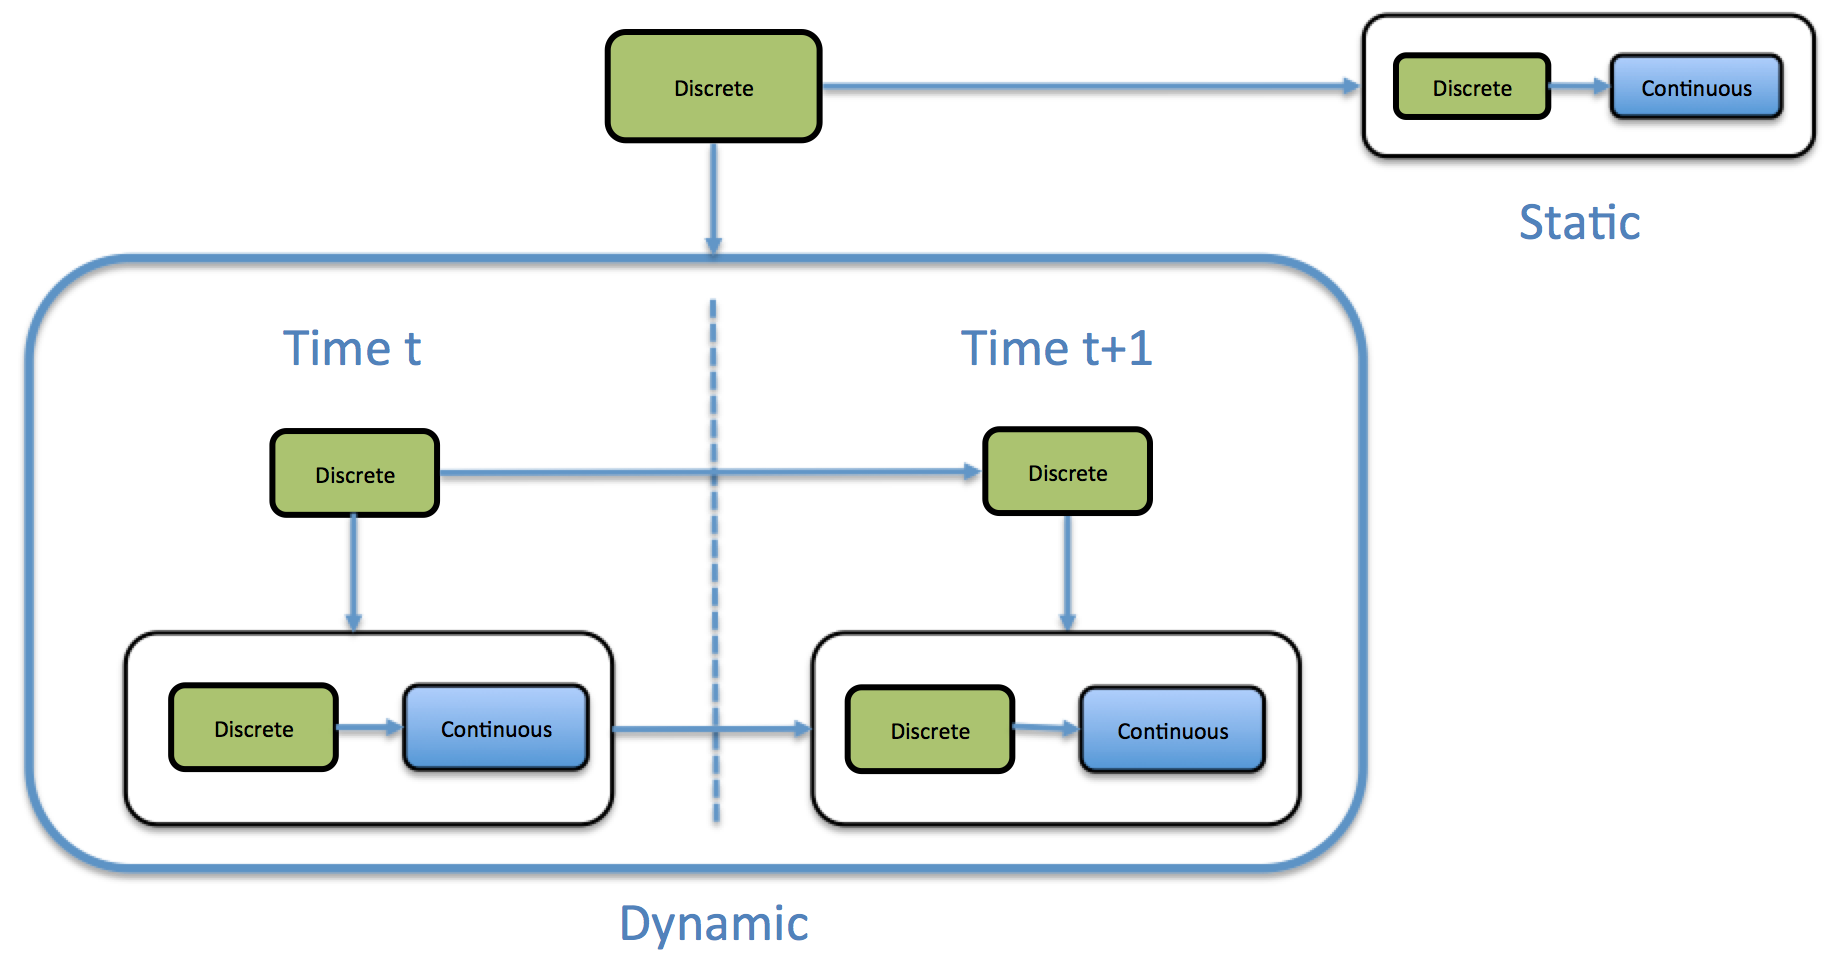
\includegraphics[scale=0.4]{./figures/CajaMarModelClass}
\end{center}
\end{figure}



\subsection{AMIDST Model Class}




\begin{figure}
\begin{center}
\caption{\label{Figure:AMIDSTModelClass} CajaMar Model Class}
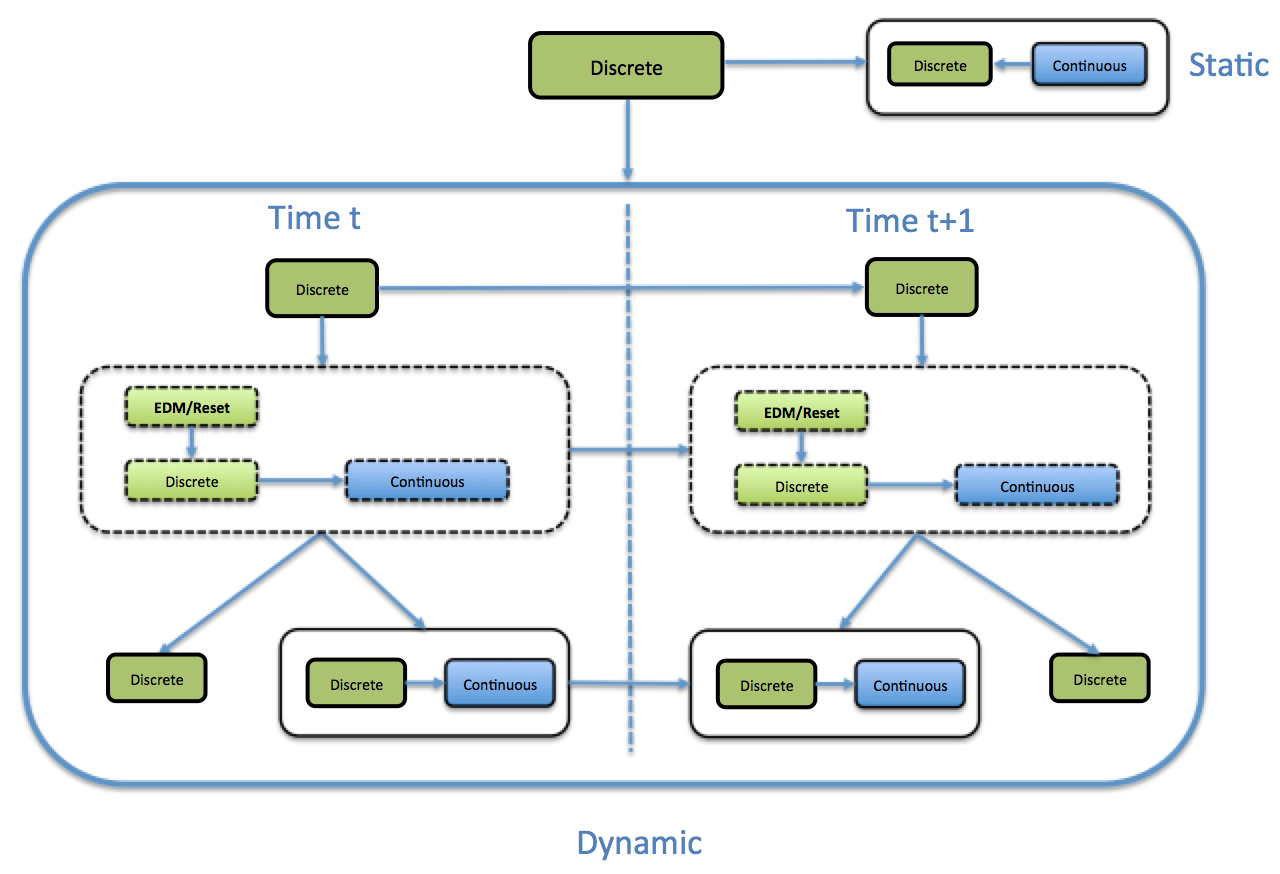
\includegraphics[scale=0.7]{./figures/AMIDSTModelClass}
\end{center}
\end{figure}